\section{Baseline Architecture}

    \begin{figure}
        \begin{center}
            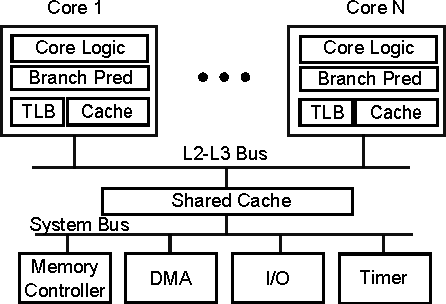
\includegraphics[width=3in]{figs/baseline.pdf}
            \caption{The timing-channel vulnerable baseline architecture.}
            \label{fig:baseline}
        \end{center}
    \end{figure}

    Figure \ref{fig:baseline} shows the baseline architecture which is later 
    extended to include timing channel protection. The architecture has 
    multiple cores, each with a branch predictor, one or more private caches, a 
    TLB, and the core logic. Each processor is connected to a shared cache 
    through an on-chip network. The multicore processor is connected to the 
    main memory and a DMA module through the system bus. 

    The hardware is concurrently shared by multiple security domains. A 
    security domain consists of one or more software modules (such as processes 
    or threads in a single OS system or virtual machines in a virtualization 
    based system). Software modules within the same security domain trust each 
    other, but information flows between security domains must be controlled 
    according to a policy that meets the security requirements of the system.
    As shown in Figure \ref{fig:baseline}, it is possible for a security domain 
    to have multiple virtual machines which may be allocated to different 
    cores. It is also possible for security domains to be time multiplexd on 
    the same core (e.g.  by context switching VMs), but it is not possible for 
    security domains to execute concurrently on the same core (e.g. through 
    SMT).

\section{Usage Scenarios and Threat Models}

    This section describes some example applications for the architecture and 
    the thread model for each usage scenario.

    \subsection{DRM Video Playback}
    Mobile devices often support applications that playback videos with various 
    DRM restrictions. For example, a user may only be able to play a video if 
    he or she has a valid subscription to the service. In this case, the 
    attacker is the owner of the mobile device who would either like to access 
    content without paying for a subscription. The adversary is capable of any 
    software attack in addition to simple physical attacks such as attempting 
    to reprogram portions of the software stack on which security depends.  
    However, physical attacks such as power side channels are too difficult or 
    expensive for the end user to carry out and therefore they are not 
    considered here.

    % I'm not sure I actually believe that the threat model should really 
    % exclude physical attacks. It seems reasonable that the adversary should 
    % at least be capable of measuring power at the pins of the SoC, but should 
    % probably not be capable of measuring signals within the chip.  Perhaps a 
    % better way to write the threat model is that the adversary *is* capable 
    % of physical attacks as well as timing channel attacks,
    % but here we extend the state of the practice to protect against timing 
    % channels since including power analysis defenses would take up too much 
    % space for one paper.
   
    \subsubsection{Baseline Security Mechanisms}
    AMD TrustZone \cite{trustzone} exemplifies a state of the practice solution 
    that can enforce these security properties, however, TrustZone does not 
    offer protection against timing channel attacks. Since the adversary can 
    carry out any software attack and timing channels can be exploited with 
    software attacks, timing channel protection is necessary to meet the 
    security requirements. 
    
    TrustZone separates the software modules into two security domains as shown 
    in Figure \ref{fig:tz_domains} . The first security domain is called the 
    normal world and it has a virtual machine that contains the operating 
    system and all user-space applications. The other security domain, the 
    secure world, contains a virtual machine that contains only a small 
    execution environment and a set of very simple libraries for handling 
    protected operations. This VM does not contain a complete operating system 
    and the libraries do not require any operating system support (e.g. they 
    may not have system calls). The secure world also contains software for a 
    simple monitor mode that handles context switching between the two domains 
    if they are time multiplexed on the same core. All of the secure world code 
    is small to reduce the chance of vulnerabilities. The secure world must 
    only allow the normal world to play the video if the subscription is valid.

    TrustZone extends the baseline cores of Figure \ref{fig:baseline} to
    those shown in Figure \ref{fig:tz_uarch}. The core logic contains a tag to 
    store which world is currently executing. To make an access to the memory 
    hierarchy, the core sends the virtual address and the current world to the 
    TLB. The TLB gets the physical address as normal (performing a page table 
    walk if needed). The physical address and current security domain are sent 
    to the cache. If the cache contains the physical address and the security 
    level of the current transaction matches the security level of the 
    transaction that brought it into the cache, the access proceeds normally.  
    Otherwise, if it is a cache miss, the cache sends the physical address and 
    the security level to the system bus to access the main memory. If the 
    security level matches the security level of the address in main memory, 
    the cache block is brought into the cache as normal and the security level 
    is tagged in the cache. If it is either a hit or a miss and the security 
    level does not meet the requirements, the access fails.

    The two virtual processors share the physical processor in time-multiplexed 
    way. Context switches may be entered either through an explicit instruction 
    or through interrupts. On a context switch, the monitor mode is entered.  
    Typically, the monitor mode will save the general purpose registers and any 
    processor configuration registers. The TLB is not flushed since the tags 
    protect illegal data accesses from happening.
%%%%%%%

    The video is sent to the device through an encrypted stream. The key used 
    for decryption is stored inside the secure world VM. To play the video, the 
    user space application must issue a special instruction to interact with 
    the secure world and decrypt the stream. This invokes the monitor mode 
    which then context switches out the normal world VM replacing it with the 
    secure world VM. The secure world VM loads the encrypted data into the 
    cache, decrypts it, and invokes the monitor to return execution to the 
    normal world. 
